\chapter{The Integer Quantum Hall Effect}
\label{ch:qhe}

A two-dimensional electron gas in a strong magnetic field shows a Hall resistance quantized to $h/\nu e^2$ with an accuracy of about one part in $10^{10}$, independent of material, geometry and disorder. This chapter builds on the Landau levels of Chapter~\ref{ch:semiclassical}. It explains what is measured, why the bulk is an insulator, how chiral edge channels carry exactly $e^2/h$ each, why disorder produces plateaus rather than destroying them, and how the effect differs from the quantum oscillations it grows out of.

Throughout, SI units are used, the electron has charge $-e$ with $e>0$, and $\cvect{B} = B\uvect{z}$. The useful scales are
\[
    \ell = \sqrt{\frac{\hbar}{eB}} \approx \frac{25.7\ \text{nm}}{\sqrt{B/\text{T}}},
    \qquad
    \omega_c = \frac{eB}{m},
    \qquad
    \Phi_0 = \frac{h}{e} \approx 4.14\times10^{-15}\ \text{T\,m}^2,
    \qquad
    \frac{h}{e^2} \approx 25.81\ \text{k}\Omega.
\]
In Gaussian units, $eB\to eB/c$, so $\ell^2 = \hbar c/eB$, $\Phi_0 = hc/e$ and $\omega_c = eB/mc$.

% ============================================================
\section{What Is Measured}
% ============================================================

\subsection{The Response Tensor in Two Dimensions}

In a two-dimensional sheet, in-plane currents respond linearly to in-plane fields:
\begin{equation}
    \begin{pmatrix} j_x\\ j_y\end{pmatrix} =
    \begin{pmatrix}\sigma_{xx} & \sigma_{xy}\\ \sigma_{yx} & \sigma_{yy}\end{pmatrix}
    \begin{pmatrix} E_x\\ E_y\end{pmatrix},
    \qquad
    \cvect{E} = \bm{\rho}\,\lvect{j},
    \qquad
    \bm{\rho} = \bm{\sigma}^{-1}.
\end{equation}
Current density in 2D is current per width, so $[\sigma] = \text{S}$ and $[\rho] = \Omega$. The combination $e^2/h$ has units of conductance, so a 2D conductivity \emph{can} be built from fundamental constants alone. (In Gaussian units a 2D conductivity is a velocity, and $e^2/h = \alpha c/2\pi$.)

\begin{theorem}[Form of the conductivity tensor]
If the system is unchanged by a $90^\circ$ rotation about $\cvect{B}$ (an isotropic gas, or a crystal with a $C_3$, $C_4$ or $C_6$ axis along $\uvect{z}$), then
\[
    \sigma_{xx} = \sigma_{yy},
    \qquad
    \sigma_{xy} = -\sigma_{yx}.
\]
\end{theorem}
\begin{proof}
The tensor must satisfy $R\bm{\sigma}R^T = \bm{\sigma}$ with $R = \begin{pmatrix}0&-1\\1&0\end{pmatrix}$, and
\[
    R\bm{\sigma}R^T = \begin{pmatrix}\sigma_{yy} & -\sigma_{yx}\\ -\sigma_{xy} & \sigma_{xx}\end{pmatrix}. \qedhere
\]
\end{proof}

Equivalently, the only isotropic responses are ``along $\cvect{E}$'' and ``rotated by $90^\circ$'': $\lvect{j} = \sigma_{xx}\cvect{E} + \sigma_H\,\uvect{z}\times\cvect{E}$. In any crystal, Onsager reciprocity $\sigma_{ij}(\cvect{B}) = \sigma_{ji}(-\cvect{B})$ makes the antisymmetric (Hall) part odd in $B$. Rotational symmetry is what removes any symmetric off-diagonal part.

\begin{formula}[Inverting the tensor]
For a tensor of this form,
\begin{equation}
    \rho_{xx} = \frac{\sigma_{xx}}{\sigma_{xx}^2+\sigma_{xy}^2},
    \quad
    \rho_{xy} = \frac{-\sigma_{xy}}{\sigma_{xx}^2+\sigma_{xy}^2},
    \quad
    \sigma_{xx} = \frac{\rho_{xx}}{\rho_{xx}^2+\rho_{xy}^2},
    \quad
    \sigma_{xy} = \frac{-\rho_{xy}}{\rho_{xx}^2+\rho_{xy}^2}.
    \label{eq:qhe-inversion}
\end{equation}
\end{formula}

\begin{fact}[Zero resistivity \emph{and} zero conductivity]
If $\sigma_{xx} = 0$ but $\sigma_{xy}\neq0$, then~\eqref{eq:qhe-inversion} gives $\rho_{xx} = 0$ as well. A quantum Hall state is simultaneously a perfect insulator ($\sigma_{xx} = 0$: no current along $\cvect{E}$) and has zero longitudinal resistance ($\rho_{xx} = 0$: no voltage drop along the current). The whole response is Hall.
\end{fact}

\subsection{The Hall Bar}

\begin{figure}[ht]
\centering
\begin{tikzpicture}[scale=1.0,>=Stealth]
  \fill[gray!12] (0,0) rectangle (7,2);
  \draw[thick] (0,0) rectangle (7,2);
  \fill[orange!40] (-0.8,0.5) rectangle (0,1.5); \draw (-0.8,0.5) rectangle (0,1.5);
  \fill[orange!40] (7,0.5) rectangle (7.8,1.5); \draw (7,0.5) rectangle (7.8,1.5);
  \node at (-0.4,1) {5}; \node at (7.4,1) {6};
  \foreach \x/\n in {2/1,5/2} {\fill[blue!30] (\x-0.25,2) rectangle (\x+0.25,2.5); \draw (\x-0.25,2) rectangle (\x+0.25,2.5); \node at (\x,2.75) {\n};}
  \foreach \x/\n in {2/3,5/4} {\fill[blue!30] (\x-0.25,-0.5) rectangle (\x+0.25,0); \draw (\x-0.25,-0.5) rectangle (\x+0.25,0); \node at (\x,-0.75) {\n};}
  \draw[<->] (2,1.55) -- node[above]{$L$} (5,1.55);
  \draw[<->] (6.3,0) -- node[right]{$W$} (6.3,2);
  \draw[->,thick,red!70!black] (0.4,1) -- (1.4,1) node[right]{$I$};
  \draw[->] (8.4,0.2) -- (9.2,0.2) node[right]{$x$};
  \draw[->] (8.4,0.2) -- (8.4,1.0) node[above]{$y$};
\end{tikzpicture}
\caption{Hall bar. Current $I$ enters and leaves at the ends (contacts 5, 6). Probes 1--4 sit on the long edges, separated by $L$; the bar has width $W$.}
\label{fig:qhe-hallbar}
\end{figure}

The long edges confine the current, so in the middle of the bar $j_x = I/W$ and $j_y = 0$. Averaging the two edges,
\begin{equation}
    E_x = \frac{V_1+V_3-V_2-V_4}{2L},
    \qquad
    E_y = \frac{V_1-V_3+V_2-V_4}{2W}.
\end{equation}
Averaging cancels, to first order, the pickup of the (large) Hall voltage by slightly misaligned longitudinal probes; symmetrizing in $\pm B$ removes the rest. With $j_y = 0$:

\begin{formula}[Hall-bar resistances]
\begin{equation}
    R_{xy} \equiv \frac{V_H}{I} = \rho_{yx} = -\rho_{xy},
    \qquad
    R_{xx} \equiv \frac{V_L}{I} = \rho_{xx}\frac{L}{W}.
\end{equation}
The Hall resistance is \emph{independent of sample dimensions}; the longitudinal one depends on the aspect ratio.
\end{formula}

Solving $j_y = 0$ gives $E_y/E_x = \sigma_{xy}/\sigma_{xx}$, and hence also $\sigma_{xy} = j_xE_y/(E_x^2+E_y^2)$.

\subsection{The Phenomenon}

At low field $R_{xy} = B/ne$ is the classical straight line of the Drude model (Section~\ref{sec:drude-hall}). At higher field it breaks into a staircase of flat plateaus, while $R_{xx}$ shows spikes only where $R_{xy}$ steps from one plateau to the next and vanishes in between.

\begin{fact}[Observed quantization]
On the plateaus,
\begin{equation}
    R_{xy} = \frac{h}{\nu e^2} = \frac{25.81\ \text{k}\Omega}{\nu},
    \qquad
    R_{xx} = 0,
    \qquad
    \nu = 1,2,3,\ldots,
\end{equation}
independent of material, geometry and disorder, and reproducible to about one part in $10^{10}$. Since 2019 the von Klitzing constant $R_K = h/e^2 = 25812.80745\ldots\,\Omega$ is exact in the SI.
\end{fact}

Even plateaus appear first, because each Landau level is spin degenerate; odd ones appear once the Zeeman splitting is resolved.

% ============================================================
\section{Landau Levels and the Incompressible Bulk}
% ============================================================

\subsection{Landau Gauge}

The free-electron Landau levels were found in Section~\ref{sec:bloch-onsager}. Here the wavefunctions matter, so we redo the calculation for the electron charge $-e$:
\begin{equation}
    H = \frac{1}{2m}\bigl(\lvect{p} + e\cvect{A}\bigr)^2,
    \qquad
    \cvect{A} = (0, Bx, 0)\ \Rightarrow\ \curl\cvect{A} = B\uvect{z}.
\end{equation}

\begin{fact}[Choosing $\cvect{A}$]
$\cvect{A} = (Bx,0,0)$ has zero curl: it is pure gauge and describes \emph{no} field. Expanding with it produces a spurious $i\hbar$ from $[\hat{x},\hat{p}_x]$. With $\cvect{A} = (0,Bx,0)$ the cross term involves $\hat{x}\hat{p}_y$, which commute, and no constant appears. In any Coulomb gauge ($\div\cvect{A} = 0$), $\hat{\lvect{p}}\cdot\cvect{A} = \cvect{A}\cdot\hat{\lvect{p}}$.
\end{fact}

$H$ is independent of $y$, so $p_y\to\hbar k$ with $\psi = e^{iky}f_k(x)$:
\begin{equation}
    H = \frac{p_x^2}{2m} + \frac12m\omega_c^2(x-x_0)^2,
    \qquad
    x_0 = -k\ell^2,
\end{equation}
a harmonic oscillator whose centre is set by $k$ (the sign of $x_0$ depends on the sign of the charge and on the gauge).

\begin{formula}[Landau levels in the Landau gauge]
\begin{equation}
    \varepsilon_n = \hbar\omega_c\bigl(n+\tfrac12\bigr),
    \qquad
    \psi_{n,k} \propto e^{iky}\,H_n\!\left(\frac{x-x_0}{\ell}\right)e^{-(x-x_0)^2/2\ell^2}.
\end{equation}
Each state is a strip: extended along $y$, localized within $\sim\ell$ of $x_0$ in $x$. The energy does not depend on $k$: each Landau level is \emph{flat}.
\end{formula}

\subsection{Degeneracy and Filling Factor}

With $k = 2\pi m/L_y$ and $0<|x_0|<L_x$, the degeneracy found in Section~\ref{sec:bloch-onsager} follows.

\begin{definition}[Filling factor]
\begin{equation}
    N_\phi = \frac{L_xL_y}{2\pi\ell^2} = \frac{B\cdot\text{Area}}{\Phi_0}\quad\text{states per level per spin},
    \qquad
    \nu = \frac{N_e}{N_\phi} = \frac{n}{eB/h} = 2\pi\ell^2n.
\end{equation}
\end{definition}

There is one state per flux quantum: each state occupies area $2\pi\ell^2$, enclosing one $\Phi_0$. Raising $B$ at fixed density $n$ lowers $\nu$, which is why the plateaus appear in the order $\ldots,6,4,2$ as $B$ increases.

\subsection{Density of States}

\begin{formula}[2D density of states in a field]
\begin{equation}
    g(\varepsilon) = g_s\frac{eB}{h}\sum_{n\ge0}\delta\!\left(\varepsilon-\hbar\omega_c\bigl(n+\tfrac12\bigr)\right),
    \qquad
    \langle g\rangle_{\hbar\omega_c} = \frac{g_sm}{2\pi\hbar^2} = g_0.
\end{equation}
\end{formula}

The field neither creates nor destroys states: the Hamiltonian acts on the same Hilbert space, and $\cvect{B}$ only changes the matrix elements. Each window of width $\hbar\omega_c$ of the zero-field continuum collapses into one degenerate level, so the average reproduces the zero-field 2D density of states $g_0$.

\subsection{Incompressibility}

At integer $\nu$ (and without disorder), $\nu$ levels are full and the next is $\hbar\omega_c$ away:
\begin{equation}
    \Delta\mu = \hbar\omega_c\ \text{(jump)},
    \qquad
    \pdv{n}{\mu} = 0,
    \qquad
    \sigma_{xx} = 0.
\end{equation}
The bulk is an \emph{incompressible} insulator. In GaAs ($m^*\approx0.067m_e$), $\hbar\omega_c\approx1.7\ \text{meV}\times(B/\text{T})$, about 20\,meV at 10\,T.

% ============================================================
\section{Edge States}
% ============================================================

\begin{figure}[ht]
\centering
\begin{tikzpicture}[scale=0.9,>=Stealth]
  \draw[thick] (0,0) rectangle (8,3.2);
  \foreach \x/\y in {2/1.6,4/1.0,5.5/2.1,3.2/2.3,6.6/1.1} {\draw[->,blue!60!black] (\x,\y) ++(0.35,0) arc (0:350:0.35);}
  \foreach \x in {0.6,1.5,...,7.3} {\draw[red!70!black,->] (\x,3.2) arc (180:360:0.45);}
  \foreach \x in {7.4,6.5,...,0.7} {\draw[red!70!black,->] (\x,0) arc (0:180:0.45);}
  \node[right] at (8.2,3.0) {\small skipping orbits};
  \node[right] at (8.2,1.6) {\small closed bulk orbits};
  \node at (4,-0.9) {\small $\cvect{B}$ out of the page};
\end{tikzpicture}
\caption{Semiclassical picture: closed cyclotron orbits in the bulk give no net motion (insulating); skipping orbits along the edges move one way (conducting), in opposite directions on the two edges.}
\label{fig:qhe-skipping}
\end{figure}

\subsection{Levels Follow the Confining Potential}

Add a confining wall $V(x)$, flat in the bulk and rising at the edges. $H$ is still independent of $y$:
\begin{equation}
    \left[\frac{p_x^2}{2m} + \frac12m\omega_c^2(x-x_0)^2 + V(x)\right]f_k = \varepsilon f_k.
\end{equation}
If $V$ varies slowly on the scale $\ell$ ($\ell|V'|\ll\hbar\omega_c$), expand about $x_0$:
\begin{equation}
    \varepsilon_n(k) \approx \hbar\omega_c\bigl(n+\tfrac12\bigr) + V\bigl(x_0(k)\bigr).
\end{equation}
Since $x_0\propto k$, a plot against $k$ is a rescaled plot against position: each level is the flat bulk value plus a copy of the wall.

\begin{figure}[ht]
\centering
\begin{tikzpicture}[xscale=1.0,yscale=1.0,>=Stealth]
  \draw[->] (-0.2,0) -- (8.4,0) node[right]{$k \propto -x_0$};
  \draw[->] (0,-0.2) -- (0,4.4) node[above]{$\varepsilon$};
  \foreach \e in {0.6,1.6,2.6} {
    \draw[thick,blue!60!black,domain=0.55:7.45,samples=80] plot (\x,{\e + 0.25*exp((\x-6.6)*1.6) + 0.25*exp((1.4-\x)*1.6)});
  }
  \draw[dashed,red!70!black] (0,2.15) -- (8,2.15) node[right]{$\varepsilon_F$};
  \foreach \x in {1.2,1.5,...,6.8} {\fill (\x,{0.6 + 0.25*exp((\x-6.6)*1.6) + 0.25*exp((1.4-\x)*1.6)}) circle (1.3pt);}
  \foreach \x in {1.5,1.8,...,6.5} {\fill (\x,{1.6 + 0.25*exp((\x-6.6)*1.6) + 0.25*exp((1.4-\x)*1.6)}) circle (1.3pt);}
  \node at (0.9,-0.45) {\small edge};
  \node at (4.0,-0.45) {\small bulk};
  \node at (7.1,-0.45) {\small edge};
\end{tikzpicture}
\caption{Landau levels against $k$ bend up at the edges, following the confining potential. Dots are occupied states; here $\nu = 2$ in the bulk, and each filled level crosses $\varepsilon_F$ once at each edge.}
\label{fig:qhe-edge-levels}
\end{figure}

\subsection{Chiral Edge Channels}

The velocity is the slope of the level with respect to $k$, so it is set by the slope of the wall:
\begin{equation}
    |v_y| = \frac1\hbar\left|\pdv{\varepsilon_n}{k}\right| = \frac{|V'(x_0)|}{eB}.
\end{equation}

\begin{fact}[Chiral edge channels]
\leavevmode
\begin{itemize}
    \item In the bulk, $V' = 0$: no velocity and no current (closed orbits).
    \item At the edges, $V'\neq0$. The wall slopes oppositely on the two sides, so the two edges move in opposite directions, and within one edge all states move the same way: the edge is \emph{chiral}.
    \item Each filled bulk level crosses $\varepsilon_F$ exactly once per edge, so there are $\nu$ channels per edge, independent of the shape of $V$.
\end{itemize}
\end{fact}

Near a crossing, $k = \pm K_n + q$ and $\varepsilon\approx\varepsilon_F\pm\hbar v_nq$: right-movers live on one edge and left-movers on the other, separated by the sample width across a gapped bulk.

% ============================================================
\section{Conductance from Edge Channels}
% ============================================================

\subsection{One Channel Carries \texorpdfstring{$e^2/h$}{e2/h}}

Fill one 1D channel by an extra $\delta\mu$. With $dk/2\pi$ states per unit length and velocity $\hbar^{-1}d\varepsilon/dk$,
\begin{equation}
    \delta I = e\int\frac{dk}{2\pi}\,\frac1\hbar\frac{d\varepsilon}{dk} = \frac{e}{h}\,\delta\mu.
\end{equation}
The velocity cancels against the 1D density of states, so the result is independent of the dispersion.

\subsection{Hall Conductance}

Let the right-moving edge be filled to $\mu_R = -eV_1$ and the left-moving edge to $\mu_L = -eV_2$. Their contributions cancel up to the lower potential, leaving

\begin{formula}[Hall conductance from edge channels]
\begin{equation}
    I_y = \nu\,\frac{e}{h}\bigl(\mu_R-\mu_L\bigr)
    \qquad\Longrightarrow\qquad
    |G_{yx}| = \nu\frac{e^2}{h}.
\end{equation}
The current flows along $y$ while the voltage is across $x$: this is a Hall conductance.
\end{formula}

\subsection{Zero Longitudinal Resistance and the Hall Bar}

Along one edge all channels share one potential, so there is no voltage drop along the current and $\rho_{xx} = 0$. In the Hall bar of Figure~\ref{fig:qhe-hallbar} (the Landauer--B\"uttiker picture), the edge leaving the source carries $\mu_S$ past probes 1 and 2, and the other edge carries $\mu_D$ past probes 3 and 4:
\begin{equation}
    V_1 = V_2,\quad V_3 = V_4\ \Rightarrow\ R_{xx} = 0;
    \qquad
    V_H = \frac{\mu_S-\mu_D}{e},\quad I = \nu\frac{e}{h}(\mu_S-\mu_D)\ \Rightarrow\ R_{xy} = \frac{h}{\nu e^2}.
\end{equation}
Dissipation occurs at the contacts (``hot spots''), not in the sample, and the two-terminal resistance is also $h/\nu e^2$, independent of length.

\begin{fact}[What did not enter]
The velocity, the shape of the wall, the mass and the sample dimensions all dropped out. The argument assumed only that (i) there is no scattering between the two edges, and (ii) scattering within one edge is harmless, since all channels there move the same way and no electron can turn around.
\end{fact}

% ============================================================
\section{Robustness and Plateaus}
\label{sec:qhe-robust}
% ============================================================

\subsection{Disorder Makes Plateaus}

Disorder broadens each Landau level. States in the centre of a broadened level remain extended; states in the tails are \emph{localized} around potential hills and valleys and carry no current.

\begin{figure}[ht]
\centering
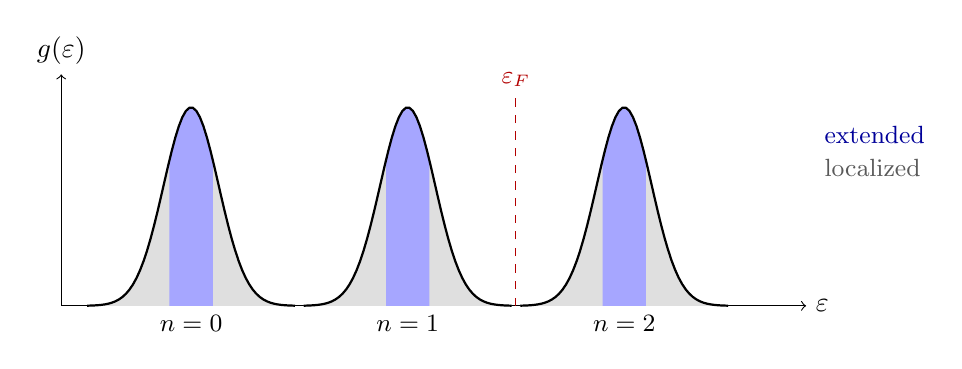
\begin{tikzpicture}[xscale=1.1,yscale=1.4]
  \draw[->] (0,0)--(8.6,0) node[right]{$\varepsilon$};
  \draw[->] (0,0)--(0,2.1) node[above]{$g(\varepsilon)$};
  \foreach \c in {1.5,4,6.5}{
    \fill[gray!25] plot[domain=\c-1.2:\c+1.2,samples=60] (\x,{1.8*exp(-((\x-\c)/0.45)^2)}) -- (\c+1.2,0) -- (\c-1.2,0) -- cycle;
    \fill[blue!35] plot[domain=\c-0.25:\c+0.25,samples=30] (\x,{1.8*exp(-((\x-\c)/0.45)^2)}) -- (\c+0.25,0) -- (\c-0.25,0) -- cycle;
    \draw[thick] plot[domain=\c-1.2:\c+1.2,samples=60] (\x,{1.8*exp(-((\x-\c)/0.45)^2)});
  }
  \draw[dashed,red!70!black] (5.25,0)--(5.25,1.9) node[above]{\small $\varepsilon_F$};
  \node[below] at (1.5,0) {\small $n=0$};
  \node[below] at (4,0) {\small $n=1$};
  \node[below] at (6.5,0) {\small $n=2$};
  \node[align=left,right] at (8.7,1.4) {\small \textcolor{blue!60!black}{extended}\\ \small \textcolor{gray!70!black}{localized}};
\end{tikzpicture}
\caption{Disorder-broadened Landau levels. While $\varepsilon_F$ moves through localized states, the number of current-carrying (extended) states below it is fixed, so $\sigma_{xy}$ stays on a plateau.}
\label{fig:qhe-broadened}
\end{figure}

As $B$ (or $n$) changes, $\varepsilon_F$ moves through localized states, which change the density but not the current. The Hall conductance stays at $\nu e^2/h$ and $\sigma_{xx} = 0$: a plateau. Only when $\varepsilon_F$ crosses the extended states at a level centre does $\sigma_{xx}\neq0$ and $\sigma_{xy}$ step. This is why the plateaus are \emph{centred} where the classical line $B/ne$ crosses $h/\nu e^2$.

\subsection{Why Disorder Cannot Spoil the Value}

Backscattering requires an electron to cross from one edge to the other through the gapped bulk, which is exponentially suppressed in the sample width. Scattering within an edge cannot reverse the direction of motion.

\subsection{Laughlin's Argument}

On an annulus, thread a flux $\Phi(t)$ through the hole. Faraday's law gives an azimuthal electric field, and a Hall conductance $\sigma_H$ moves charge radially: $\Delta Q = \sigma_H\,\Delta\Phi$. After one flux quantum the Hamiltonian returns to itself (gauge invariance), and with a bulk gap only an integer number of electrons can have moved between the edges.

\begin{theorem}[Laughlin]
\begin{equation}
    \Delta Q = \nu e\quad\text{for}\quad\Delta\Phi = \Phi_0 = \frac he
    \qquad\Longrightarrow\qquad
    \sigma_H = \nu\frac{e^2}{h}.
\end{equation}
\end{theorem}

This uses only gauge invariance and the gap. The integer is a topological invariant of the occupied states (the TKNN integer).

% ============================================================
\section{Integer Quantum Hall Effect versus Quantum Oscillations}
% ============================================================

Both phenomena come from the same Landau levels and the same Onsager quantization (Sections~\ref{sec:bloch-onsager} and~\ref{sec:bloch-dhva}). They differ in dimension, in regime, in what is measured, and above all in what controls the answer.

\subsection{Same Levels, Different Consequences}

\paragraph{Three dimensions.} Each Landau level disperses along $\cvect{B}$, $\varepsilon_n(k_z) = \hbar\omega_c(n+\tfrac12) + \hbar^2k_z^2/2m$, so
\begin{equation}
    g_{3D}(\varepsilon) \propto \frac{eB}{h}\sum_n(\varepsilon-\varepsilon_n)^{-1/2},
    \qquad
    \frac{\delta g_{3D}}{g_{3D}} \sim \left(\frac{\hbar\omega_c}{\varepsilon_F}\right)^{1/2} \ll 1.
\end{equation}
There is never a gap. The system stays metallic, and only a small oscillating fraction of states, near the extremal orbit, responds coherently.

\paragraph{Two dimensions.} There is no $k_z$: the levels form a comb, $\delta g/g\sim1$, and $\varepsilon_F$ can sit in a true gap. This is the precondition for $\sigma_{xx} = 0$ and a quantized $\sigma_{xy}$.

\paragraph{One sample, both effects.} In a 2D sample at low field ($\nu\gg1$), the levels are dense and overlapping: $\rho_{xx}$ shows Shubnikov--de Haas oscillations periodic in $1/B$, and $\rho_{xy}$ is close to the classical line. As $B$ grows, $\hbar\omega_c$ exceeds the level broadening, gaps open between the levels, and the SdH minima deepen to $\rho_{xx} = 0$ while $\rho_{xy}$ develops plateaus. Quantum oscillations are the weak-field precursor of the quantum Hall effect.

\subsection{Comparison}

\begin{table}[ht]
\centering
\small
\renewcommand{\arraystretch}{1.25}
\begin{tabular}{p{2.8cm}p{5.4cm}p{5.4cm}}
    \toprule
    & \textbf{Quantum oscillations (dHvA, SdH)} & \textbf{Integer quantum Hall effect}\\
    \midrule
    Dimension & Mostly 3D metals (also 2D at low $B$) & 2D only\\
    Regime & Many levels filled ($\nu\gg1$); $\hbar\omega_c\ll\varepsilon_F$ & Few levels filled; $\varepsilon_F$ in a gap\\
    Observable & Small periodic modulation of $M$, $\chi$, $\rho_{xx}$ & Flat plateaus in $\rho_{xy}$; $\rho_{xx} = 0$ exactly\\
    Field dependence & Periodic in $1/B$: $F = \hbar A_{\text{ext}}/2\pi e$ & Steps between plateaus; plateau values do not depend on $B$\\
    What it measures & Fermi-surface geometry: extremal areas, $m^*$, $\tau_q$, Berry phase $\gamma$ & The universal constant $e^2/h$ times an integer\\
    Material dependence & Everything is material-specific & None: universal to $10^{-10}$\\
    Role of disorder & Damps the amplitude ($R_D = e^{-\pi p/\omega_c\tau_q}$) & Needed for the plateau \emph{width}; cannot change the value\\
    Role of temperature & Damps the amplitude ($R_T = X/\sinh X$, sets $m^*$) & Activated: $\rho_{xx}\propto e^{-\Delta/2k_BT}$ on plateaus\\
    Which states matter & Extremal orbits on the Fermi surface & Chiral edge channels; extended bulk states between plateaus\\
    Underlying principle & Onsager area quantization & Gauge invariance + gap $\Rightarrow$ topological integer\\
    \bottomrule
\end{tabular}
\caption{Quantum oscillations and the integer quantum Hall effect compared.}
\label{tab:qhe-vs-qo}
\end{table}

\begin{fact}[The essential distinction]
Quantum oscillations are a \emph{spectroscopy}: their frequency, amplitude and phase encode details of the band structure, and every one of them changes from material to material. The integer quantum Hall effect is a \emph{quantization}: in the gapped regime the Hall conductance counts filled levels (more precisely, a topological invariant of the occupied states) and is insensitive to every microscopic detail. The same Landau-level spectrum produces both; whether the Fermi level sits inside a broad continuum of states (oscillations) or inside a gap (quantization) decides which one is seen.
\end{fact}

\begin{fact}[Summary of key formulas]
\begin{align*}
    &\varepsilon_n = \hbar\omega_c\bigl(n+\tfrac12\bigr),\quad N_\phi = \frac{B\cdot\text{Area}}{\Phi_0},\quad \nu = \frac{nh}{eB} && \text{Landau levels}\\
    &g(\varepsilon) = g_s\frac{eB}{h}\sum_n\delta(\varepsilon-\varepsilon_n) && \text{2D density of states}\\
    &\sigma_{yx} = -\sigma_{xy} = \nu\frac{e^2}{h},\ \sigma_{xx} = 0;\quad \rho_{xy} = \frac{h}{\nu e^2},\ \rho_{xx} = 0 && \text{quantization}\\
    &\delta I = \frac{e}{h}\,\delta\mu\ \text{per channel},\quad \nu\ \text{channels per edge} && \text{edges}\\
    &\Delta Q = \sigma_H\,\Delta\Phi,\quad \Delta\Phi = \Phi_0\Rightarrow\Delta Q = \nu e && \text{Laughlin}
\end{align*}
\end{fact}
